% GigaScience template
\documentclass[a4paper,num-refs]{oup-contemporary}

\journal{gigascience}


%%%% Packages %%%%
\usepackage{siunitx}
\usepackage{minted} % Used for JSON highlighting
\usepackage{algpseudocode} % Algorithmic environment
\usepackage{xspace}
\usepackage{booktabs}

%%%%%%

\usepackage{xcolor}
\usepackage{graphicx}
\usepackage{algorithm}
\usepackage{caption}
\usepackage{subcaption}
\usepackage{listings}
\usepackage{verbatim}
\usepackage{makecell}
\usepackage[flushleft]{threeparttable}

\usepackage{subcaption}
\usepackage{xspace}
\usepackage{stmaryrd} % for llbracket and rrbracket
\usepackage{amsmath}
\DeclareMathOperator*{\argmin}{argmin}

%%%% Commands %%%%
\newcommand{\todo}[1]{\color{red}\textbf{TODO:}#1\color{black}}
\newcommand{\note}[2]{\color{blue}Note: #1\color{black}}
\newcommand{\reprozip}[0]{ReproZip\xspace}
\newcommand{\tristan}[1]{\color{blue}\textbf{From Tristan:}#1\color{black}}

 
\title{NURM: a tool to 
locate numerical differences in pipelines}
  
\begin{document}

\author[1]{Ali Salari}
\author[1]{Lalet Scaria}
\author[2,3]{Gregory Kiar}
\author[2]{Lindsay Lewis}
\author[2,3]{Alan C. Evans}
\author[1]{Tristan Glatard}

\affil[1]{Department of Computer Science and Software Engineering, Concordia University, Montreal, Canada}
\affil[2]{McGill University, Montreal, Canada}
\affil[3]{Montreal Neurological Institute, Montreal, Canada}

\maketitle

\begin{abstract} 

Many experiments show that computational analysis results are still not 
completely reproducible. Computational environments including different 
operating systems, hardware categories, and software versions are known 
to have effects on the results produced by analysis pipelines. These 
effects are presumably due to the creation, propagation and 
amplification of small numerical differences across the pipelines. 
Although new techniques such as virtualization, version control 
systems, and provenance management tools provide more reliable 
environment and significantly improve the reproducibility of scientific 
findings. However, the precise causes of such instabilities and the 
path along which they propagate in the pipelines are unclear.  We 
present a technique to identify the processes in the pipeline that 
create numerical differences along the execution, and we apply this 
technique to the HCP structural pre-processing pipelines.

\end{abstract}

\begin{keywords}
Reproducibility; Numerical Instability; Neuroimaging.
\end{keywords}

\section{Introduction}

A reproducible study provides a context in which one is able to get 
results that are consistent with the original 
work~\cite{plesser2018reproducibility}. Research findings are expected 
to be reproducible so that their authenticity and reliability can be 
evaluated. 

Reproducibility is defined as the ability to regenerate the same 
results as the original findings when the experiment is reanalyzed by 
exactly the same analytic methods, software package, parameters, and 
data~\cite{peng2011reproducible}. 

In addition, numerical reproducibility is defined as the ability to 
regenerate bit for bit identical results from multiple 
runs~\cite{hill2017numerical}. This Numerical reproducibility can be 
checked by comparing the binary content of the results which is 
computed by the checksum method.
Regarding these definitions, it must be pointed that a
computation might be reproducible, but not 
be numerically reproducible. For instance, small numerical differences 
created during the pipeline execution may hamper numerical 
reproducibility, but be negligible in the final results.

Recently, scientists began to realize that the results of many 
scientific experiments were not reproducible. According to the previous 
studies, variety of computational infrastructures including workstation 
types, parallelization methods, operating systems, and analysis 
packages are known to influence reproducibility~\cite{Gronenschild2012, 
diethelm2012limits, Glatard2015, bowring2019exploring}.

In particular, the effect of operating system is quantified 
in~\cite{Glatard2015, Gronenschild2012} specially on some of the main 
neuroimaging pipelines including FSL, CIVET and Freesurfer pipelines. 
The binary differences are measured by the checksum method between 
results of the same analyses on different operating systems, which 
indicate a significant disparity. 

This irreproducibility issues are reported as the result of the 
creation, propagation, and amplification of small numerical 
differences~\cite{Gronenschild2012, diethelm2012limits, Glatard2015, 
bowring2019exploring}. In this case, the analysis pipelines are said to 
be numerically unstable. Numerical instability is a characteristic of 
the pipelines which amplify small numerical differences and then hamper 
the reproducibility of the analyses depending on the length of the 
pipeline and magnitude of the differences. In many cases, numerical 
instability is an important issue for reproducibility.

There are different solutions to make reproducible analysis including 
containerization techniques that encapsulate software/hardware 
dependencies, provenance capturing tools, and version control systems. 
However, a comprehensive solution requires to fix the numerical 
instabilities. For this purpose, we introduce a Numerical 
Reproducibility Measurement (NURM) tool to identify the processes in 
pipeline that create numerical differences across several runs. In this 
paper, the execution results of pipelines across different operating 
systems are considered to find out the cause of the irreproducibility 
using the interposition techniques.

The remainder of this paper describes the NURM-tool in different parts 
including the way of capturing and representation of the provenance 
information, the method of clustering of different subject types, and 
process labelling to characterize differences. We describe the HCP 
preprocessing pipelines as a popular neuroimaging project to test the 
NURM-tool and evaluate its functionality. Finally, we reported the 
experimental results which describe the processes that are responsible 
for the differences in the pipelines.

\tristan{define subjects, explain neuroimaging, bring context.}
\section{Tool description}

Figure~\ref{fig:overview} shows an overview of our method. For
each tested condition, the pipeline is containerized with Docker, and its
interface is described with Boutiques~\cite{glatard2017boutiques}.
\reprozip~\cite{Chirigati2016} is added to one of the container images for
provenance tracking. 
Our tool starts by capturing temporary and multi write files in condition 1 
(Fig.~\ref{fig:overview-capturing}). 
To do that, the tool first executes pipeline on condition 1 to obtain process graph 
(Fig.~\ref{fig:overview-capturing} - (P)) and 
result files. Subsequently, it generates the list of processes that create these intermediary files. 
Using this list, the tool modifies docker image in condition 1 and exectutes the pipeline 
again through it, which turns to produce results including temporary and overwritten
files (Fig.~\ref{fig:overview-capturing} - (C1)).
In the second step, the processes are labeled from 
the differences found in their outputs in the
two tested conditions (Fig.~\ref{fig:overview-labelling}). To this order, 
the tool builds docker image for condition 2 by modifying pipeline processes that 
recognised from 
the process graph. Then, the modified docker image is executed in condition 2 and 
each process is labeled right 
after the running by comparing checksum of the results obtained in condition 1 
and output files of the process in condition 2 (Fig.~\ref{fig:overview-labelling} - (D)). 
We then label processes in 3 categories (Fig.~\ref{fig:overview-labelling} -
(L)) depending whether they create differences (represented in red) or not (green). 
Process labelling is done through hooks which are defined during the docker image modifying procedure, 
and incremental updates in condition 2, 
until the end of the pipeline execution.

\begin{figure}
  \centering
  \begin{subfigure}{\columnwidth}
    \centering
    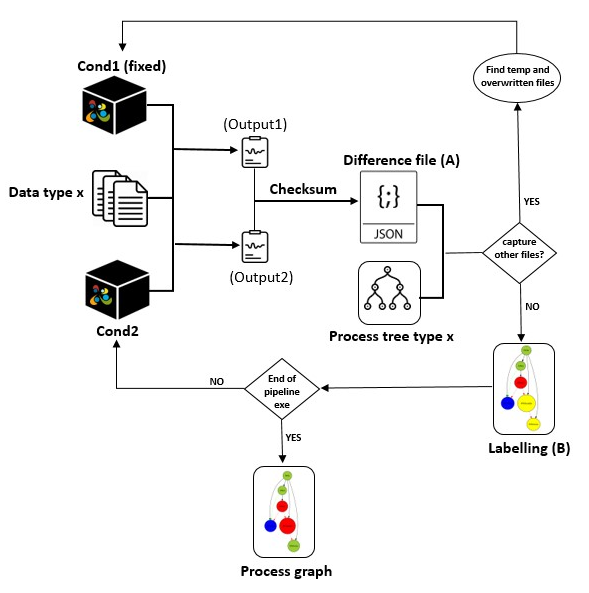
\includegraphics[width=1\columnwidth]{images/Slide2}
    \caption{Capturing of temp and multi write files.}
    \label{fig:overview-capturing}
  \end{subfigure}
   \begin{subfigure}{\columnwidth}
    \centering
     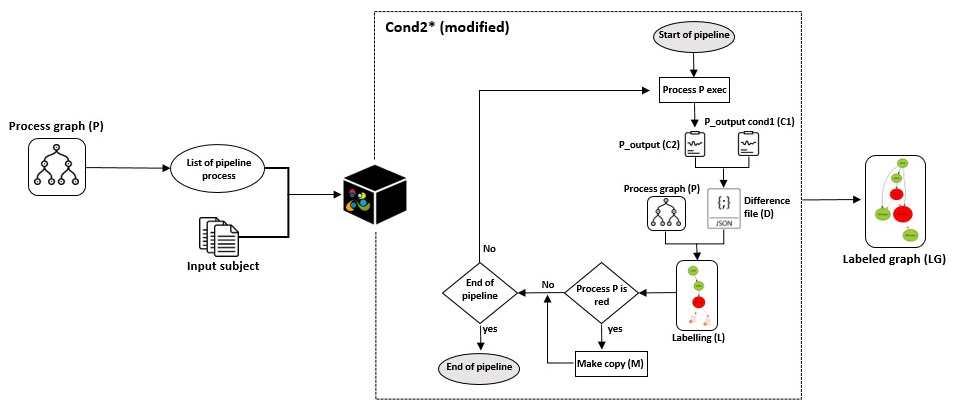
\includegraphics[width=1\columnwidth]{images/Slide1}
     \caption{Process labelling.}
     \label{fig:overview-labelling}
   \end{subfigure}
   \caption{Method overview}
   \label{fig:overview}
  \end{figure}

\subsection{Provenance capture and representation}

We use \reprozip to create process graph (Fig.~\ref{fig:overview-capturing} - (P)), 
which records: (1) the set of processes created by the
pipeline, using the \texttt{clone()} or \texttt{fork()} system call, and
(2) the set of files read, written and executed by each process, including
temporary files. \reprozip collects this information through the
\texttt{ptrace()} system call and stores it in a SQLite database.

Our tool reconstructs a process tree starting from the first process
created by the pipeline and traversing processes through \texttt{clone()}
and \texttt{fork()}. It also creates a process \emph{graph} from this tree
by adding edges corresponding to file dependencies between processes. A
file dependency is defined between processes A and B if a file written by A
is read by B. Figure~\ref{fig:simple_script} shows an example of a process
tree and graph constructed from the example pipeline in
Listing~\ref{listing:sample-script}.
\begin{listing}
\begin{minted}[frame=single,
  framesep=3mm,
  linenos=false,
  xleftmargin=0pt,
  tabsize=4]{bash}
#!/bin/bash
if [ #$ !=1 ]
then
    echo "usage: 0 <inputimage.nii.gz>"
    exit 1
fi

# Parse argument, set file names
input_image=$1
bet_output="$(basename ${input_image} 
                       .nii.gz)_brain.nii.gz"
bet_output_binarized="$(basename ${input_image} 
                       .nii.gz)_brain_bin.nii.gz"

# Run FSL bet, put result ${bet_output}
bet ${input_image} ${bet_output} > bet_temp.out
echo "Voxels / Volume in brain mask:"
# Run FSL stats on ${bet_output}
fslstats ${bet_output} -V
# Run FSL maths on ${bet_output}
fslmaths ${bet_output} ${bet_output_binarized}
echo "Voxels / Volume in binarized brain mask:"

\rm bet_temp.out
\end{minted}
  \caption{Example pipeline}
  \label{listing:sample-script}
\end{listing}

\begin{figure}
\centering
  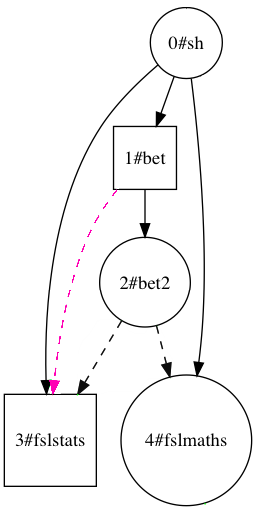
\includegraphics[scale=0.25]{images/simple_graph}
  \caption{Process tree and graph
  constructed from the example pipeline in
  Listing~\ref{listing:sample-script}.
  Processes that read or write
  temporary files are 
  represented with squares. Plain edges 
  represent the process tree (\texttt{fork()} or \texttt{clone()} 
  system calls). Dashed edges represent file dependencies: temporary 
  files are in yellow and result files are in green.
  Every node in the tree is labeled using (1) a process id created by our
  reconstruction, (2) the name of the executable run by the process.
  Process 0 is the initial call to the \texttt{bash} interpreter, and
  processes 1, 3 and 4 are the calls to FSL bet, stats and maths made in
  Listing~\ref{listing:sample-script}. Process 2 is forked by process 1: it
  was captured by \reprozip while it did not appear in
  Listing~\ref{listing:sample-script}. 
}
  \label{fig:simple_script}
\end{figure}


\subsection{Graph analysis}

We label in two categories the processes of the graph of each subject:
\begin{enumerate}
\item Processes that read files that do not have differences and write files that do not have differences 
are labeled \emph{transparent} (Figure~\ref{fig:processes}.a).
\item Processes that read files 
that do not have differences but write files that have differences 
\emph{create} differences (Figure~\ref{fig:processes}.b).
\end{enumerate}

In addition, there are two more situations in labelling process as:
\begin{enumerate}
\item Processes that read files 
that have differences and write files that do not have differences \emph{remove} 
differences (Figure~\ref{fig:processes}.c).
\item Processes that read files that have differences and write files that 
also have differences are called
\emph{undetermined} (Figure~\ref{fig:processes}.d).
\end{enumerate}

\begin{figure}%\centering
\centering
    \begin{subfigure}{0.2\linewidth}
        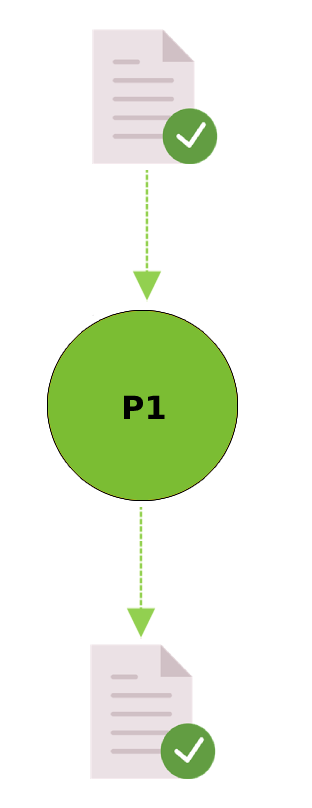
\includegraphics[scale=0.3]{images/green.png}
        \caption{Transparent}
        \label{fig:green}
    \end{subfigure}
    \hfill
    \begin{subfigure}{0.2\linewidth}
    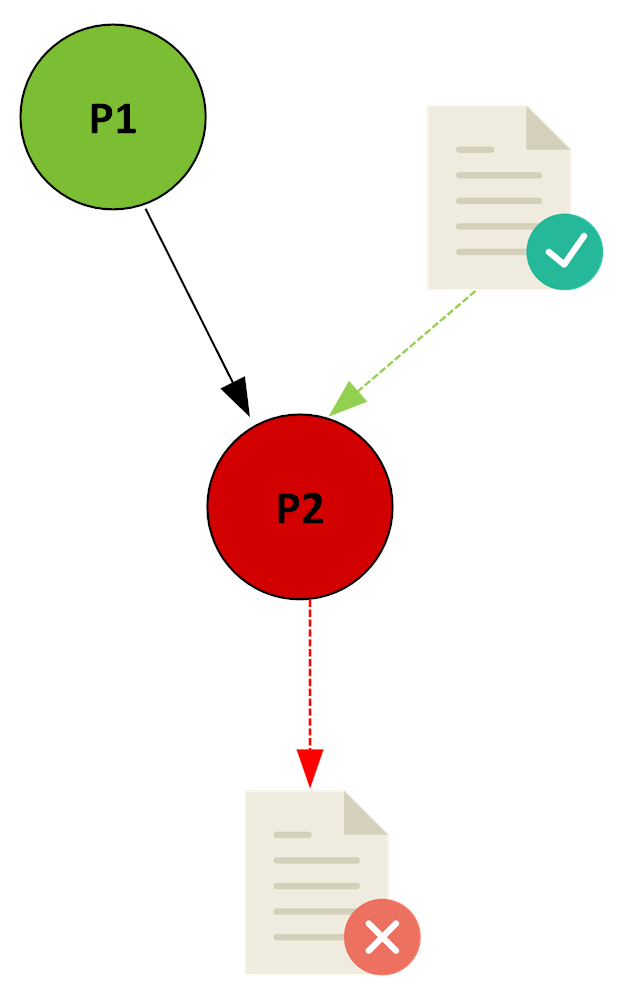
\includegraphics[scale=0.3]{images/red.png}
    \caption{Creates differences}
    \label{fig:red}
    \end{subfigure}
    \hfill
    \begin{subfigure}{0.2\linewidth}
    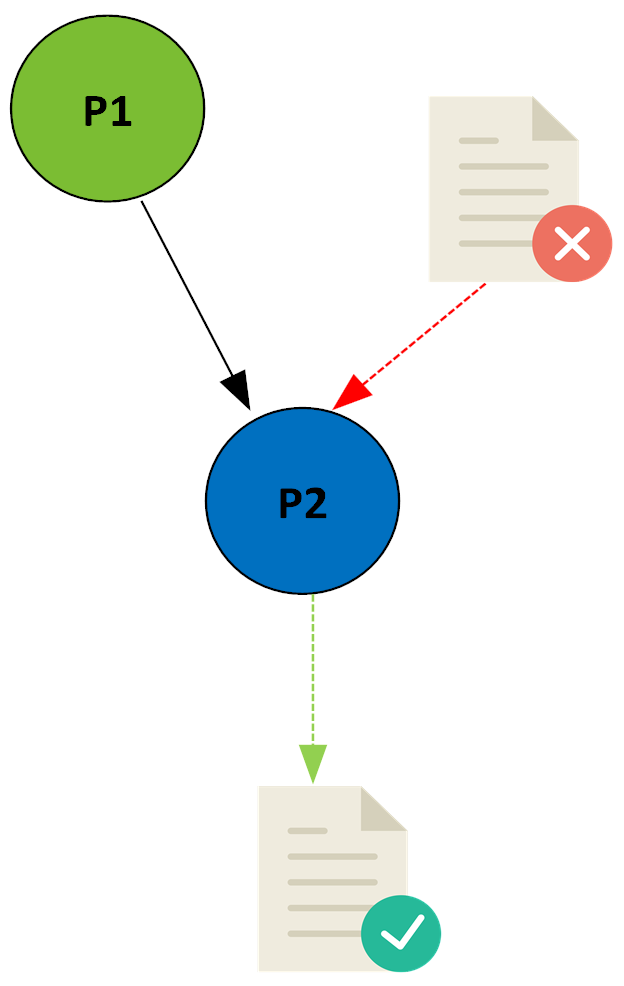
\includegraphics[scale=0.3]{images/blue.png}
    \caption{Removes differences}
    \label{fig:blue}
    \end{subfigure}
    \hfill
    \begin{subfigure}{0.2\linewidth}
    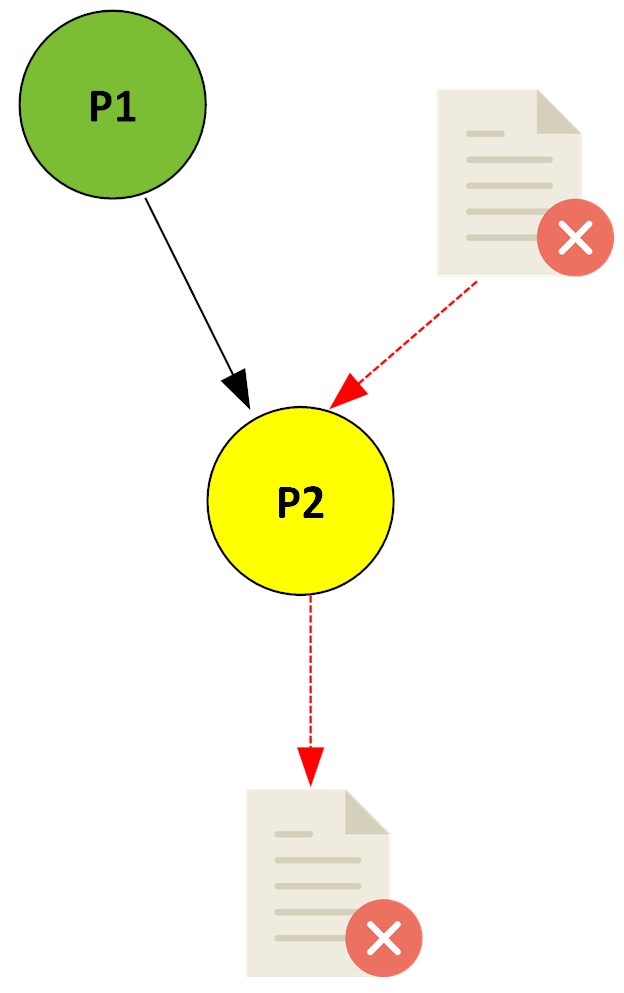
\includegraphics[scale=0.3]{images/yellow.png}
    \caption{Undetermined}
    \label{fig:yellow}
\end{subfigure}
    \caption{Different type of labeled process based on the input/output files.
  Dashed edges refer to the file dependencies between processes A and B 
  if a file written by A is read by B. Solid black edges refer to the 
  relationship between parent and child processes.}
    \label{fig:processes}
\end{figure}

Undetermined processes are due to temporary files, and files that were
written by more than a single process. In both situations, hooks must
be added to the pipeline to capture intermediary file states and label
undetermined processes.

\subsubsection{Capturing temporary files} 

The labelling of processes that read or 
write temporary files is undetermined because these files are deleted during 
the execution. To address this issue, we replace in Condition 1 every process P that 
writes temporary files with a modification of P that first calls P and then
backs up all its output files to a read-only directory. This replacement is
done by modifying the PATH environment variable to point to a directory
containing a modified version of the executable called by the process. The
modified executable will run the original executable and then backup its
output files. \tristan{Add an example modified script (listing), and replace input checks on file names by checksums.}
This 
solution does not cover the temporary files that are removed by P 
itself, but this is not a problem since these files do not play any role in 
the subsequent steps of the pipeline. 

\subsubsection{Capturing multiple write files}

Files written by multiple processes also lead 
to undetermined labels. For a file F 
written by all processes in \textbf{P} = \{$P_{1}$, \ldots $P_{n}$\}, we 
(1) check that processes in \textbf{P} do not write concurrently to F, 
(2) we establish an order on \textbf{P} based on the creation timestamp 
of the processes, (3) we replace every process $P_{i}$ in \textbf{P} by 
a wrapper that first calls $P_{i}$ and then backs up F to a read-only 
directory \tristan{add example of wrapper}. Thus, multiple versions of F are saved and used in the 
analysis. 

Furthermore, cycles may be present in the process graph in case a file 
was written by more than one process. We remove such cycles by removing 
file edges between processes A and B when A's process creation 
timestamp is posterior to B's or when A=B. Indeed, such edges cannot 
happen in practice unless A and B were running concurrently, which we 
assume is not the case (the tool checks for that). 

After that all these modifications are done, we re-execute pipeline in condition 1.
Figure~\ref{fig:overview-capturing} - (C1) shows pipeline results including intermediary files 
captured as the outputs in condition 1.

\subsubsection{Labelling undetermined processes} 

Since all the result files are captured in condition 1, the tool 
is ready to label the piepeline processes based on the results in condition 2.
However, another challenge is to label undetermined processes that read files with 
differences and write files with differences too. In such 
situations, it is not possible to determine from the pipeline results 
whether the process created differences, removed some differences, or 
was transparent.
To address this issue, we set hooks in the pipeline 
in Condition 2. Hooks are set by replacing We identify dall the pipeline 
processes with a custom script. This custom script labels each process 
as \emph{transparent} or \emph{create differences} immediately after running 
the original executable. 
The replacement is done through the PATH variable, as before. Moreover, 
this custom script copies the results obtained from the same process in 
Condition 1 to the pipeline output in Condition 2 if 
it is invoked with 
the arguments of a process that created differences. 
Differences are identified by comparing process name and checksum of the output files.
We developed an incremental approach that consists of the following steps: 

\begin{enumerate}
  \item Start the pipeline execution in Condition 2; 
        after hooking all the processes involved in the pipeline.
  \item Label each process as \emph{transparent} or \emph{create differences} 
        right after its running (Fig.~\ref{fig:overview-labelling} - (L)).
  \item Check if process is \emph{create differences} then: 
        copies the results produced by the same process in Condition 1 to the 
        pipeline output in Condition 2 (Fig.~\ref{fig:overview-labelling} - (M)). 
  \item Continue steps 2 and 3 until the end of the pipeline execution.
\end{enumerate}

This algorithm create a labeled process graph at the end of pipeline execution 
(Fig.~\ref{fig:overview-labelling} - (LG)).

\begin{figure}
  \centering
  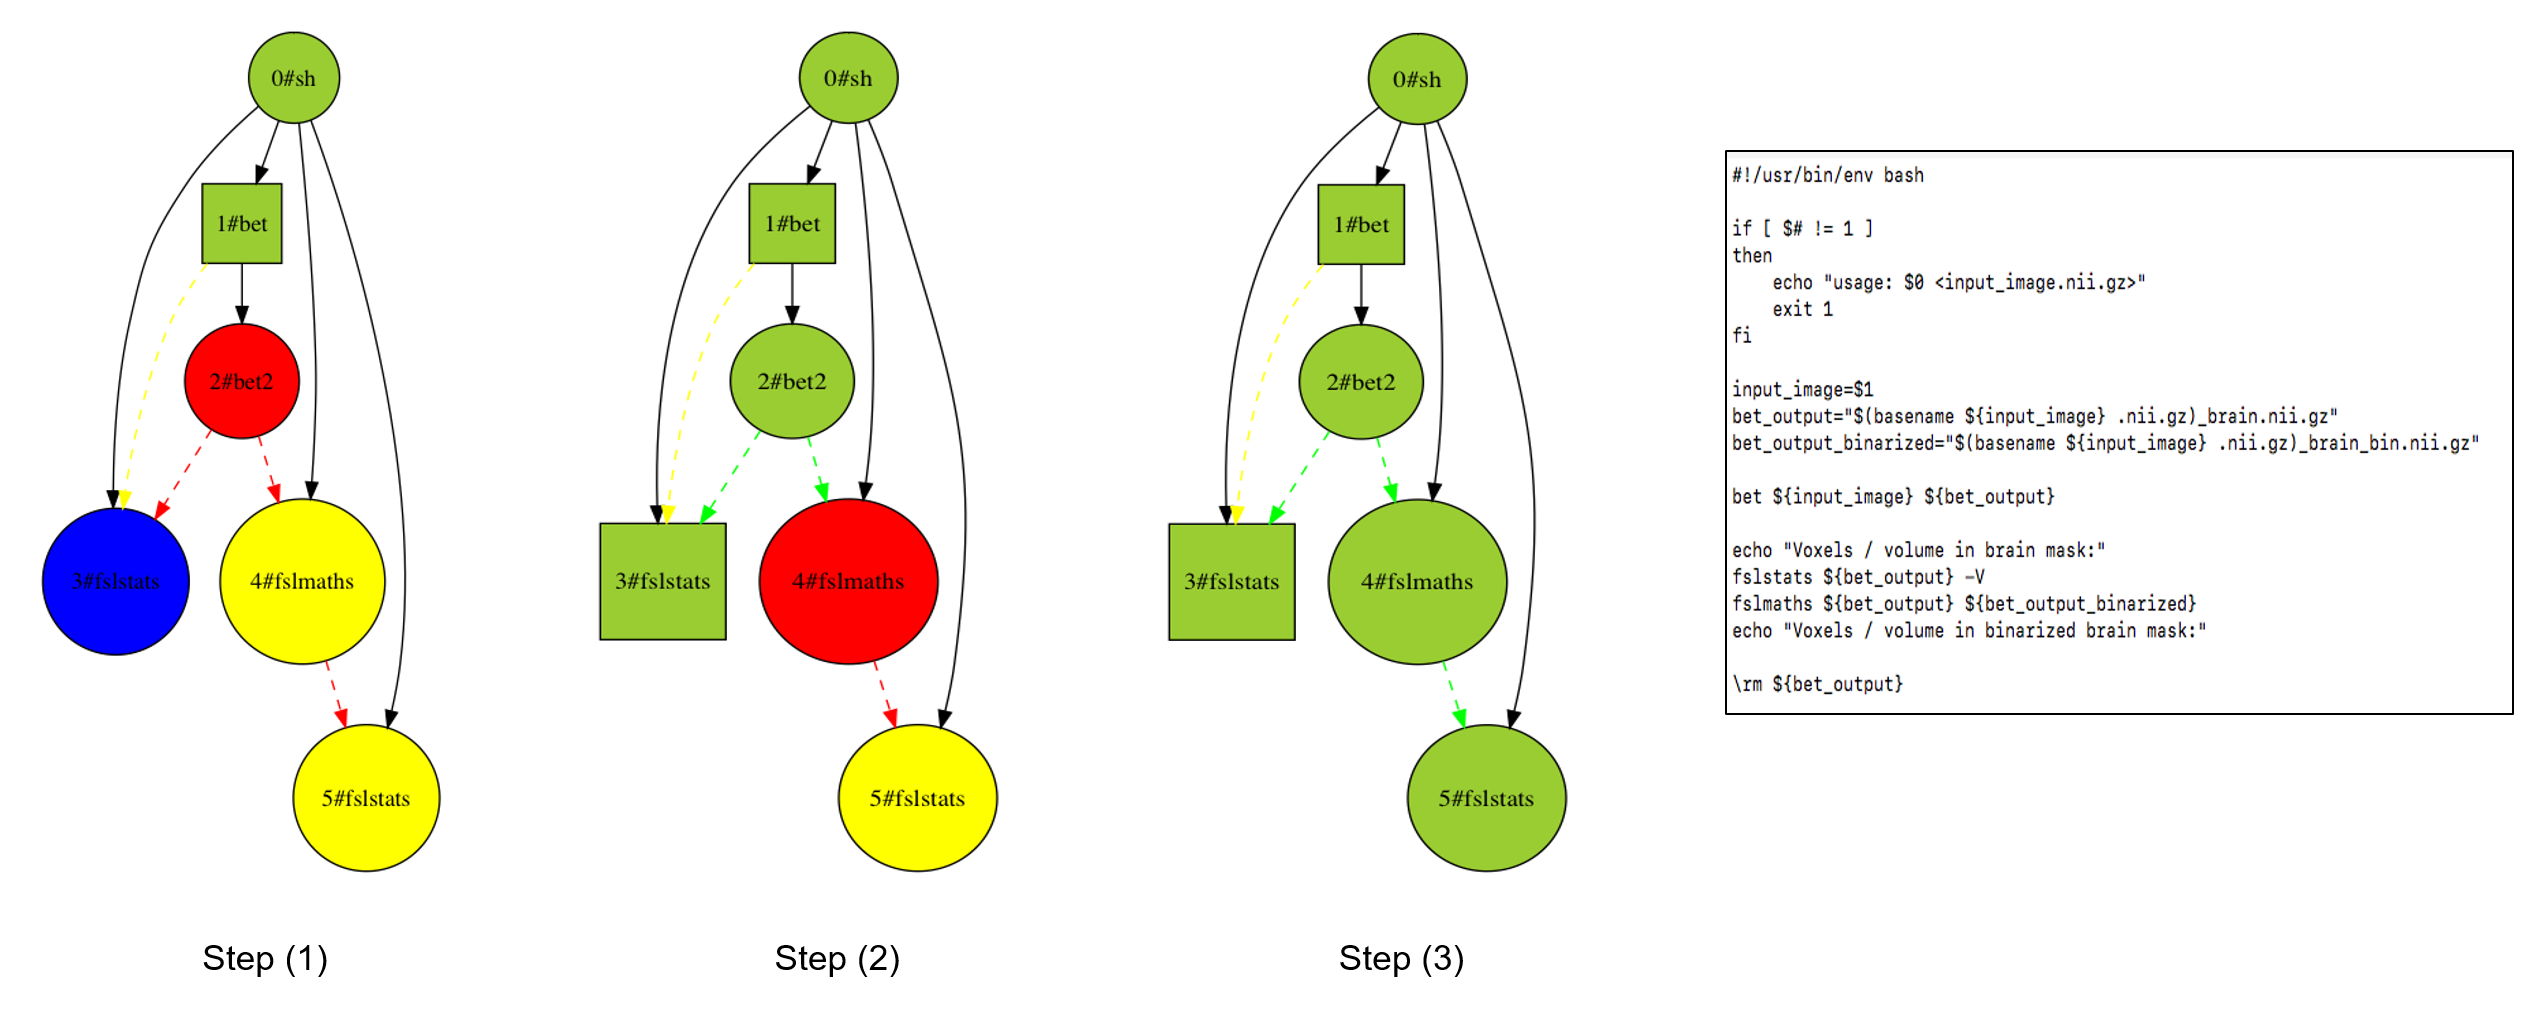
\includegraphics[width=\columnwidth]{images/iterative_modif}
  \caption{A simple example of steps of the proposed approach.}
  \label{fig:iterations}
\end{figure}

Figure~\ref{fig:iterations} illustrates our incremental labelling 
process for the example in Figure~\ref{fig:simple_script}. At every 
step, processes that created differences are shown in red and other processes 
(transparent processes) are in green. As in 
Figure~\ref{fig:simple_script}, plain black edges represent the process 
tree and dashed edges represent file dependencies: green edges 
represent files with no differences, while red edges represent files with 
differences. Temporary files are not represented because they have been 
backed up as previously described.

The four steps in Figure~\ref{fig:iterations} correspond to the 
steps of the labelling algorithm. 
At step one, process \texttt{1\#bet} is executed and then labeled 
as transparent (green) as it produced files without differences.
At step 2, \texttt{2\#bet2} 
is labeled as difference creator (red) as it produced files with differences 
from files without differences. Therefore, the files produced by \texttt{2\#bet2} in  
condition 2 are replaced with the files produced by \texttt{2\#bet2} in 
condition 1.
At step 3, after running process \texttt{3\#fslstats}, it labeled as 
transparent as it write files without differences.
At step 4, process \texttt{4\#fslmaths} is labeled as difference creator 
as the last process of the pipeline.
As a result of these 4 steps, the final process labelling is: 
\texttt{2\#bet2} and \texttt{4\#fslmath} are difference creators (red) 
and the other processes are transparent.
It should be noted that process that remove differrences are not recognised 
by this method.

\subsection{Subject clustering}

Different subjects may lead to different process trees and graphs, due to
variations that may be coming from differences in data types or
cardinality. For instance, some images may have been acquired multiple
times in some subjects. Some of these differences can be neglected, for
instance when a data decompression step is present at the beginning of the
execution for some subjects only, and other ones cannot, when different
processing paths are used in different subjects.

To address this issue, we use the tree edit distance~\cite{zhang1989simple}
to measure the distance between labeled trees \tristan{how about graphs?
also, why between \emph{labeled} trees and not just trees?}, defined as the
minimum weighted \tristan{weighted by what?} number of edit operations
required to transform one tree into the other one. Three edit operations
are considered: node label modification, node removal, and node insertion.
Each operation has an associated cost: 1 for insertion and removal, and
either 1 or 2 for label modification depending on the type of modification. \tristan{Please check my edits.}

With this distance, we cluster subjects using agglomerative hierarchical
clustering as implemented in SciPy~\cite{oliphant2007scipy}
(Algorithm~\ref{algo:hclustering}). As a result, the distance between
any two subjects in a cluster is lower than a threshold parameter.

\begin{algorithm}[h!]
\caption{Hierarchical clustering algorithm from SciPy}
\label{algo:hclustering}
\begin{algorithmic}

  \State /* Input: - a list of n trees; \texttt{T = [t${_1}$, t${_2}$,...,t${_n}$]}
  \State /*\quad \quad \quad \quad - a distance threshold value; \texttt{threshold}
  \State /* Output: a list of clusters; \texttt{C = [c${_1}$,c${_2}$,...,c${_k}$]}
  \State \texttt{\# Create a cluster for each tree in input list;}
  \State \texttt{C = [ [t${_1}$], [t${_2}$], \ldots , [t${_n}$] ]}
  \State \texttt{\# Define a 2 $\times$ 2 array to store distances}
  \State \texttt{D} = \texttt{array(n, n)}
  \While{\texttt{len(C)} > \texttt{1}}  
  \State \texttt{\# Select the two nearest clusters}
  \For{\texttt{i=1} to \texttt{n}}
  \For{\texttt{j=i+1} to \texttt{len(C)}}
  \State \texttt{D[i][j]} = \texttt{edit\_distance(C[i], C[j])} \tristan{how do you define the distance between two clusters?}
    \EndFor
  \EndFor
  \State \texttt{i, j} = $\argmin \left\{ \texttt{D[i][j]}, \ \texttt{i, j} \in \llbracket 1, \texttt{len(C)}\rrbracket^2 \right\}$
  \If{\texttt{D[i][j]} > \texttt{threshold}}
  \State \Return \texttt{C}
  \Else
  \State \texttt{\# Merge C[j] into C[i]}
  \State \texttt{C[i]} = \texttt{merge}(\texttt{C[i] and C[j]})
  \State \texttt{\# Remove C[j] from C}
  \State \texttt{remove(C[j], C)}
  \EndIf
  \EndWhile
%  \State Function edit\_distance (C${_1}$, C${_2}$)
%  \State EndFunction
\end{algorithmic}
\end{algorithm}

\tristan{how do you choose the representative process graph in each cluster?}

\section{Experiments}

\tristan{Add section introduction. Talk about OS}

\subsection{HCP pipelines and datasets}

\tristan{Add introduction on HCP project and data}

The Human Connectome Project (\href{https://www.humanconnectome.org}{HCP})
developed a set of pre-processing pipelines to process structural,
functional and diffusion MRI data acquired in the project. We focus on HCP
pre-processing pipelines for structural data, in particular PreFreesurfer
and Freesurfer. A detailed description of the analyses done in the
pipelines is available in~\cite{glasser2013minimal}.
% IF NEEDED, ADD MORE DETAILS ABOUT WHAT THE PIPELINES DO
% The structural pre-processing pipelines consists of PreFreeSurfer, 
% FreeSurfer and PostFreeSurfer. In this paper, 
% we analyzed PreFreeSurfer pipeline which consist of various steps 
% including correction of MR 
% gradient nonlinearity distortions, align the T1w and T2w images using 
% FSL FLIRT, Align native space to MNI template using ACPC and FSL FLIRT, 
% brain extraction usin FSL FLIRT and FNIRT to MNI template, register T2w 
% to T1w using FLIRT's BBR, perform a bias field correction, and register 
% the subject's native structural space to MNI space.

In these experiments, we first quantify the effect of Linux version on
these pipelines. Then we use our NURM tool to identify the processes in the
pipelines that are responsible for such effects.

We randomly selected 100 subjects from the HCP data release S500 and then 
using the NURM-tool we cluster them into different groups. 
Figure~\ref{fig:subj-clusters} shows the result of data clustering. 
Among our dataset, we identified 4 types of subjects with 
different topology of process trees. In addition, we verified that 
the process trees were identical for all subjects of the same type in 
different versions of CentOS operating system. The remainder of the 
analysis is done separately for each subject type.

%\begin{figure}
%\centering
%  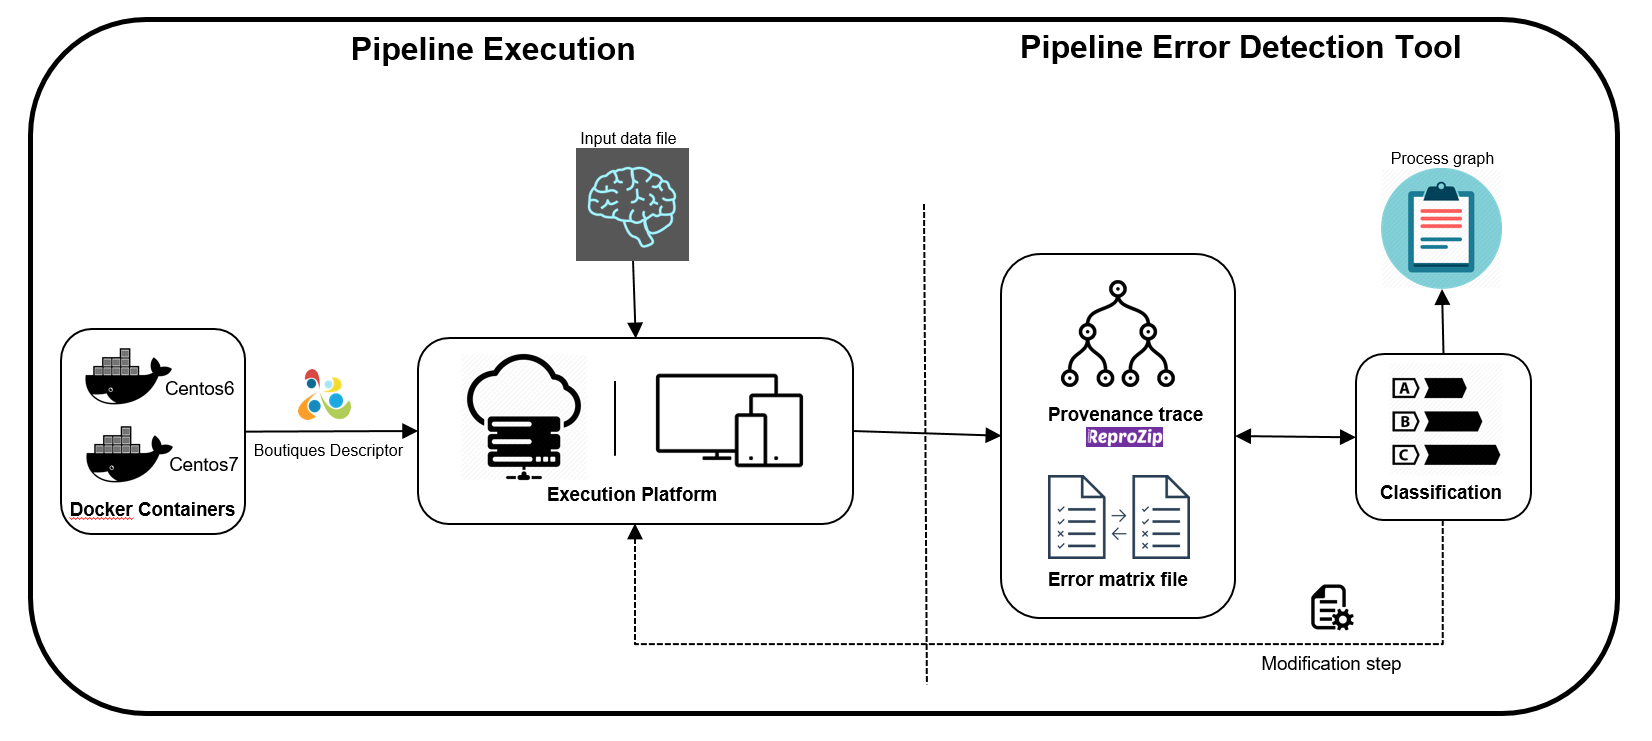
\includegraphics[width=\columnwidth]{images/overview.png}
%  \caption{An overview of the proposed technique.}
%  \label{fig:overview}
%\end{figure}


%\begin{table}
%\centering
%\begin{threeparttable}
%\caption{An overview of the HCP data (Humman Connectome DB).}
%
%\begin{tabular}{@{}llllll@{}}
%\toprule
%Subject & Release & Acquisition & Gender & Age      & Subj\_Type   \\ \midrule
%103515  & Q1      & Q02         & F      & 26-30    & type1         \\
%105216  & Q3      & Q03         & M      & 26-30    & type4         \\
%103414  & Q2      & Q02         & F      & 22-25    & type1         \\
%125525  & Q1      & Q01         & F      & 31-35    & type1         \\
%142828  & Q1      & Q01         & M      & 31-35    & type1         \\
%129533  & Q3      & Q04         & F      & 31-35    & type1         \\
%103818  & Q1      & Q01         & F      & 31-35    & type3         \\
%133928  & Q2      & Q03         & M      & 26-30    & type3         \\
%148032  & Q3      & Q03         & F      & 31-35    & type2         \\
%139637  & Q2      & Q03         & F      & 31-35    & type1         \\ \bottomrule
%\end{tabular}
%\begin{tablenotes}
%      \small
%      \item *Subj\_Type refers to the tree topology type of the subjects.
%\end{tablenotes}
%\end{threeparttable}
%\label{table:data}
%\end{table}



\subsection{Results}

We executed the pipelines using Docker containers to simplify the 
deployment of different operating system versions on execution 
platforms. The Docker images were built for the HCP PreFreeSurfer 
pipeline v3.19.0 in 
CentOS 6.8 and CentOS 7.2. Docker images are available on DockerHub for 
reuse \url{https://hub.docker.com/r/bigdatalabteam/hcp-prefreesurfer/}. 

Two types of errors can occur in the subjects due to the 
errors in the operating systems. One is inter-OS error caused by the 
operating system library updates and the other type, intra-OS errors 
occurs as a result of the pseudo-random processes used in the 
pipelines. An example of a pseudo-random process function is, a random 
number generator that would get initialized using a seed state. the 
proposed method can be used to identify both kind of errors. The files 
that are common to all the subjects only are taken into consideration 
for comparison. The first step is identification of files with 
differences in their checksums. This is identified using the checksums 
that are recorded after the processing. Intra-OS errors are identified 
using the run-number added as the suffix for the conditions. For 
example, the two batches of subjects processed under the same condition 
(CentOS6) are stored as run-1 and run-2. The files belonging to the 
subjects stored under the above mentioned conditions are treated as 
intra-OS runs.


\subsubsection{Inter-OS binary differences}


In the previous study~\cite{Scaria2017}, we showed that pre-processing 
pipelines of the Human Connectome Project~\cite{Glasser2013} were 
sensitive to operating system variation so that Figure 
\ref{fig:tissue_class} illustrates the binarized errors after brain 
tissue segmentation process in FreeSurfer. In addition, 
Figure~\ref{fig:fnirt_result} shows the same errors occurred in 
non-linear registration process between CentOS6 and CentOS7 in PreFreeSurfer. 

\begin{figure}
%  \includegraphics{brain\_classification}
\centering
  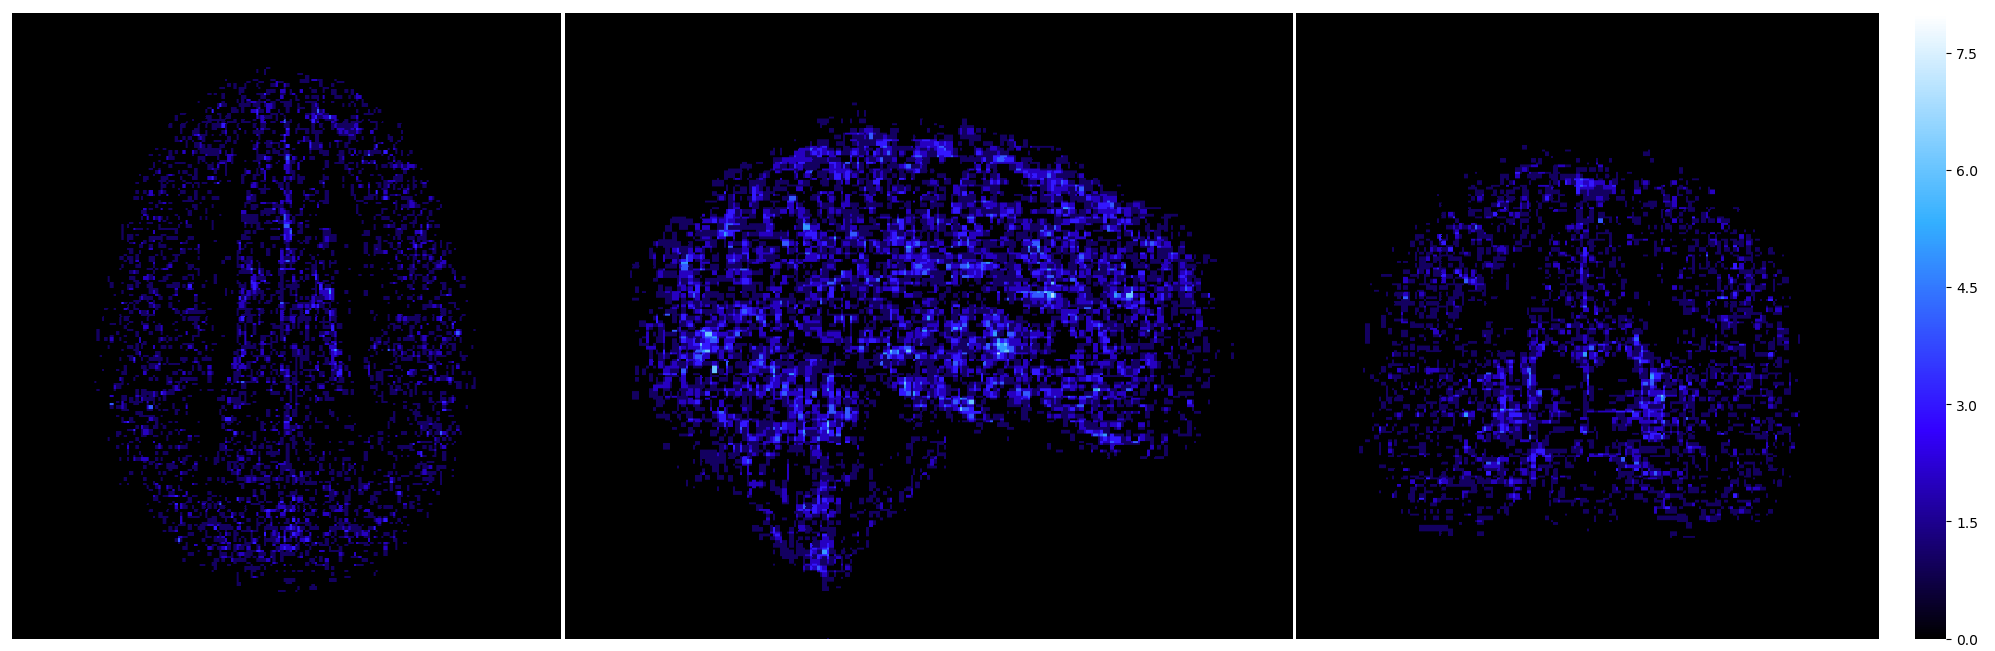
\includegraphics[width=\columnwidth]{images/brain_classification.png} 
  \caption{Binarized error between brain segmentation results from 
  FreeSurfer, subject 105216 (CentOS6 vs. CentOS7)~\cite{Scaria2017}.
    } 
  \label{fig:tissue_class}
\end{figure}

\begin{figure}
\centering
  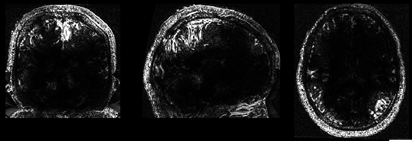
\includegraphics[width=\columnwidth]{images/fnirt_result.png} 
  \caption{Absolute errors between FNIRT results from PreFreeSurfer 
  (T2w\_acpc\_to\_MNI\_nonli.nii.gz), subject 104820 (CentOS6 vs. 
  CentOS7)~\cite{Scaria2017}. } 
  \label{fig:fnirt_result}
\end{figure}

\subsubsection{PreFreeSurfer pipeline analysis} 

We identified processes that introduce errors in PreFreeSurfer 
pipeline. Among the 117 data files produced by PreFreeSurfer, 21 did 
not have any error for any subject, 92 had errors for all subjects and 
4 had errors for 3 subjects only. 

Figure \ref{fig:complete-graph} shows the annotated provenance graph 
of the PreFreeSurfer pipeline executed on CentOS6 and CentOS7. Each 
node in the graph represent an executed process in the pipeline. 
Processes that created errors are shown in red, processes that removed 
errors are in blue, and other processes are in green.  Squares denote 
processes for which the labelling is uncertain, due to temporary 
files that were removed during the execution. Black edges link 
sub-processes to their parents while dashed edges denote file 
dependencies between processes (green edges: files with no errors; red 
edges: files with errors; yellow edges: temporary files).

The processes that introduce errors in PreFreeSurfer along with the 
number of occurrences are depicted in Figures~\ref{fig:pfs_table, 
fig:pfs_chart} including linear registration with “\emph{FLIRT}” (in 
ACPC Alignment, BrainExtraction, DistortionCorrection, 
AtlasRegistration), non-linear registration with “\emph{FNIRT}” (in 
BrainExtraction and AltasRegistration), image warping with 
“\emph{new\_invwarp}” (in BrainExtraction and AtlasRegistration).  In 
addition, errors were observed in image mean and standard-deviation 
computations with “\emph{fslstats}” (in BiasFieldCorrection), and in 
masked image extrapolation with “\emph{fslmaths}” (in 
BiasFieldCorrection).  Besides, transformation format conversion with 
“\emph{convertwarp}” (in DistortionCorrection) was able to remove 
errors.

\begin{figure}
\centering
  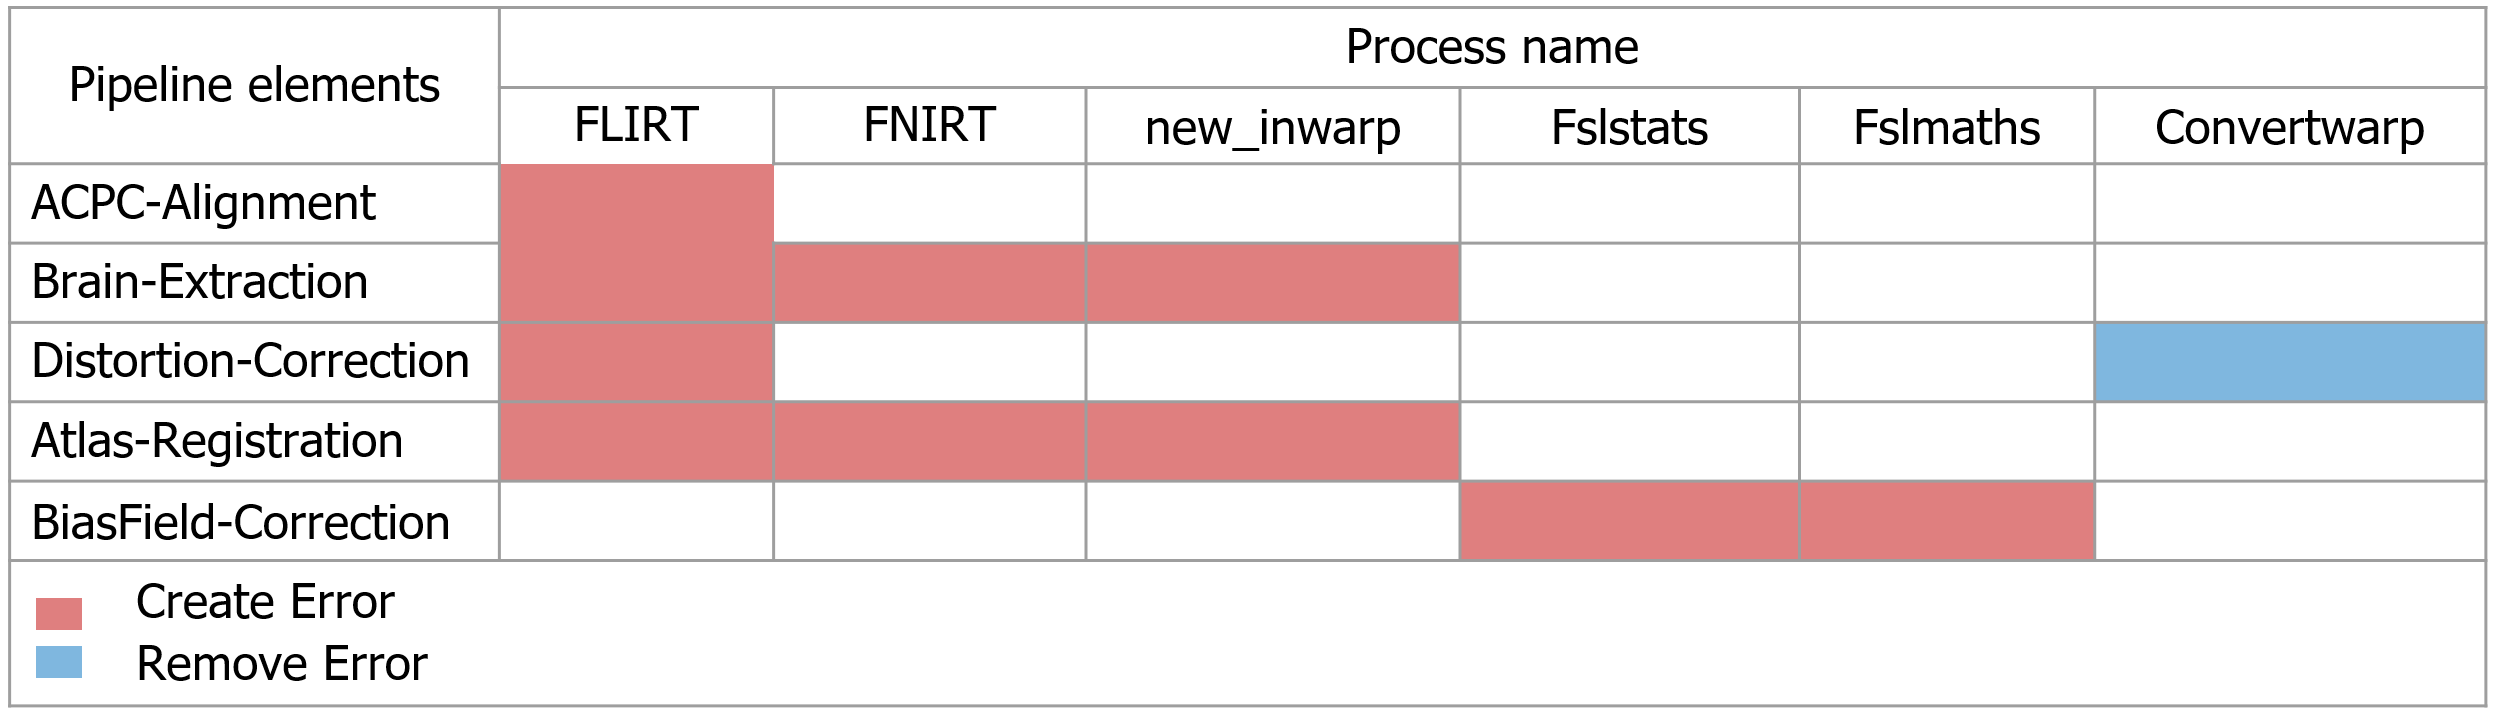
\includegraphics[width=\columnwidth]{images/pfs_table.png}
  \caption{Process name along with the pipeline elements that introduce 
  errors.}
  \label{fig:pfs_table}
\end{figure}

\begin{figure}
\centering
  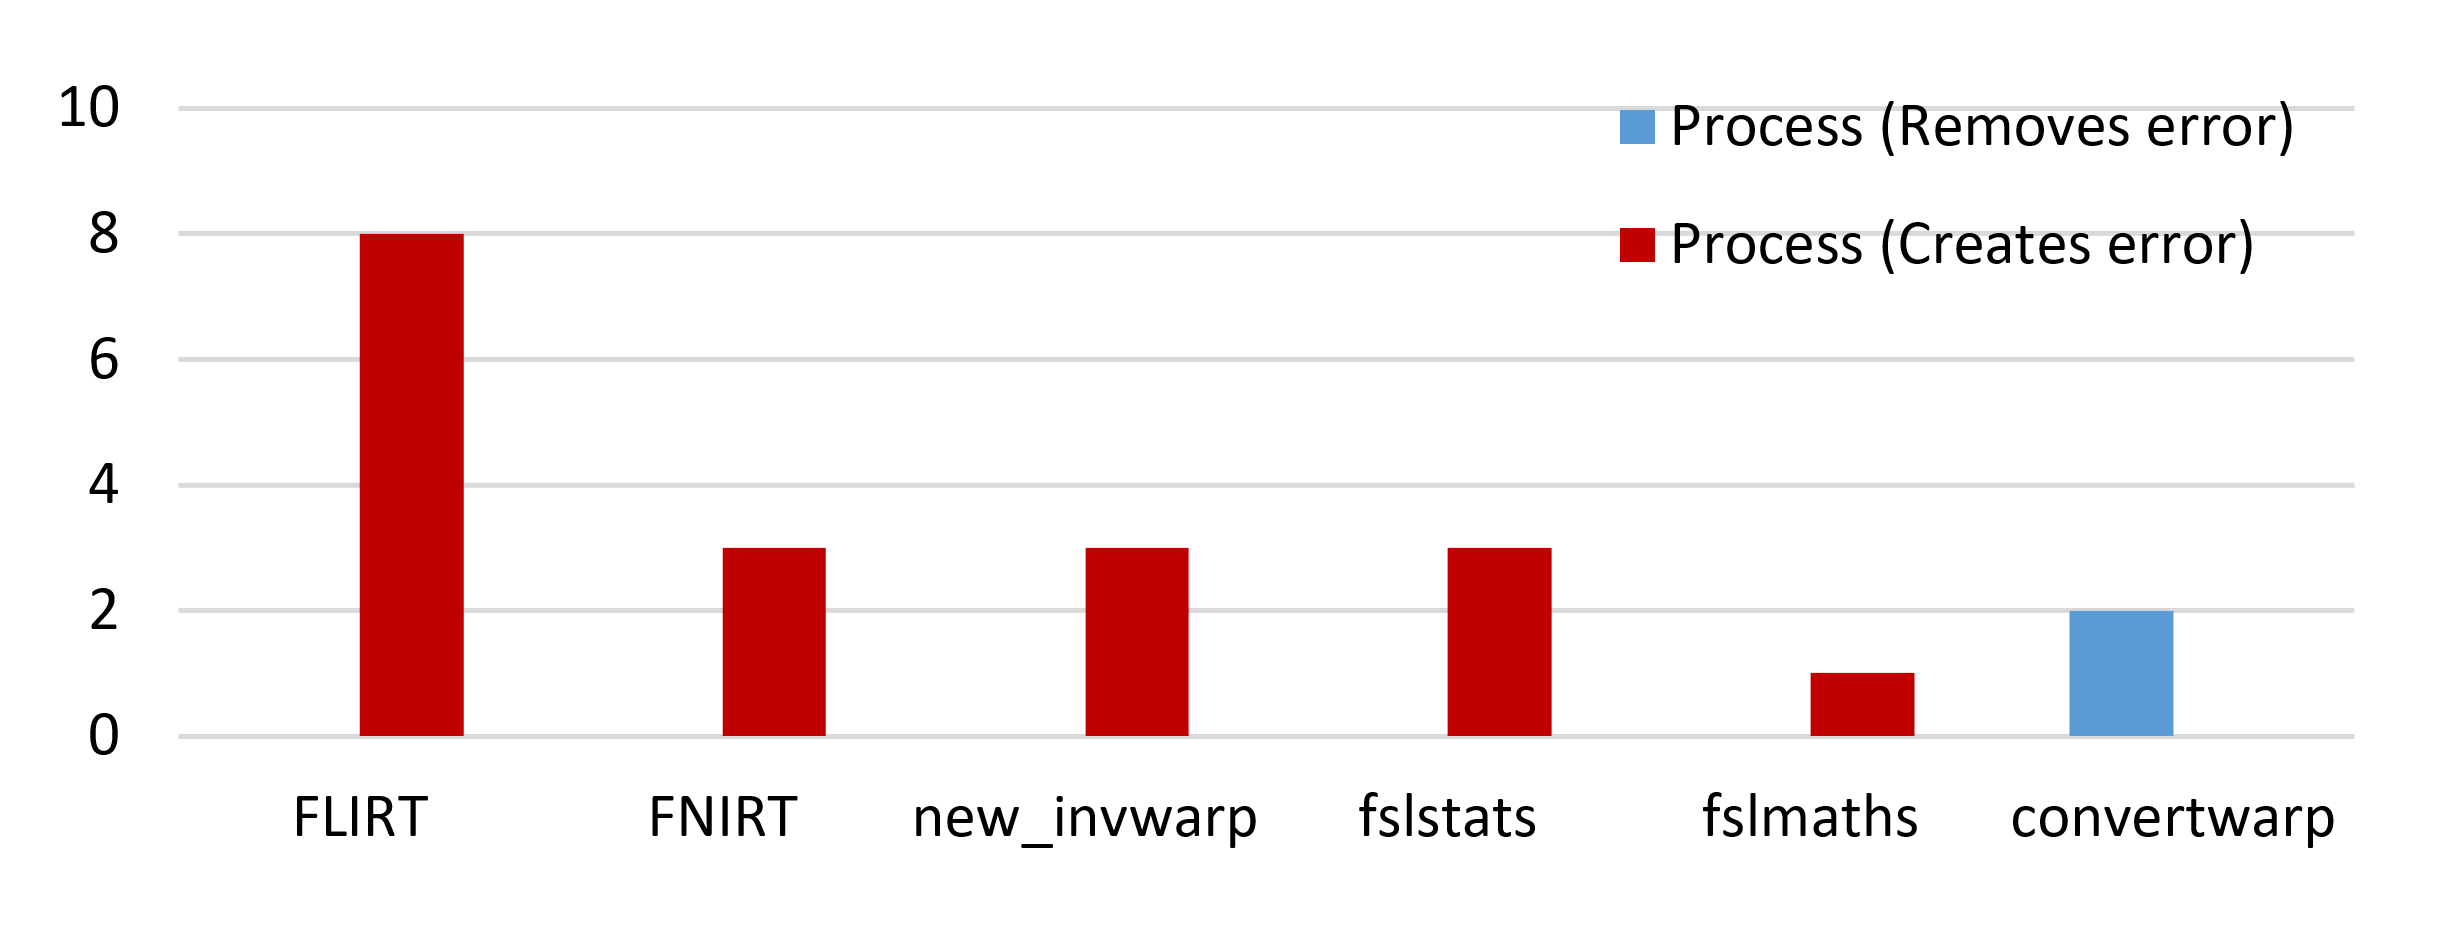
\includegraphics[width=\columnwidth]{images/pfs_chart.png} \caption{Number 
  of occurrences of errors in PreFreeSurfer on subject 103515, red and 
  blue bars indicate the processes which create and remove errors 
  respectively.} 
  \label{fig:pfs_chart}
\end{figure}


\section{Discussion}

\note{Pipeline amplify small numerical differences because they are numerically 
unstable. Furthermore, math libraries evolve over time, leading to 
different numerical errors. we listed some of the irreproducibility 
causes of the pipelines as we mentioned in the previous section 
overally along with exact command arguments.

Mention that this was only possible because the unprocessed data was 
shared in the first place. DICOM to Nifti conversion was out of scope 
and may introduce other issues.}

\section{Conclusion}

\note{Our technique is able to characterize the stability of a pipeline's 
components automatically. The numerical instability in the 
PreFreesurfer HCP pipeline arises mainly from linear and non-linear 
registration processes implemented in FSL FLIRT and FNIRT. 

There are a few ways to impede such instabilities:
\begin{itemize}
\item Use a single operating system
\item Containerize pipelines
\item Increase numerical precision
\item Be stricter on truncation and rounding standards (IEEE 754)
\item Build static executable
\end{itemize}

The results still suffer from small perturbations literally because of 
the fact that pipeline are not numerically stable. The preferred 
solution is to detect and fix numerical instability of the pipeline 
instead of masking the problem. These processes need to be reviewed to 
understand and correct the cause of instabilities. }


\section{Acknowledgments}

Data were provided by the Human Connectome Project, WU-Minn 
Consortium (Principal Investigators: David Van Essen and Kamil Ugurbil; 
1U54MH091657) funded by the 16 NIH Institutes and Centers that support 
the NIH Blueprint for Neuroscience Research; and by the McDonnell 
Center for Systems Neuroscience at Washington University.

\note{CBRAIN team. Compute Canada(Calcul Quebec).}

\begin{figure*}
\centering
  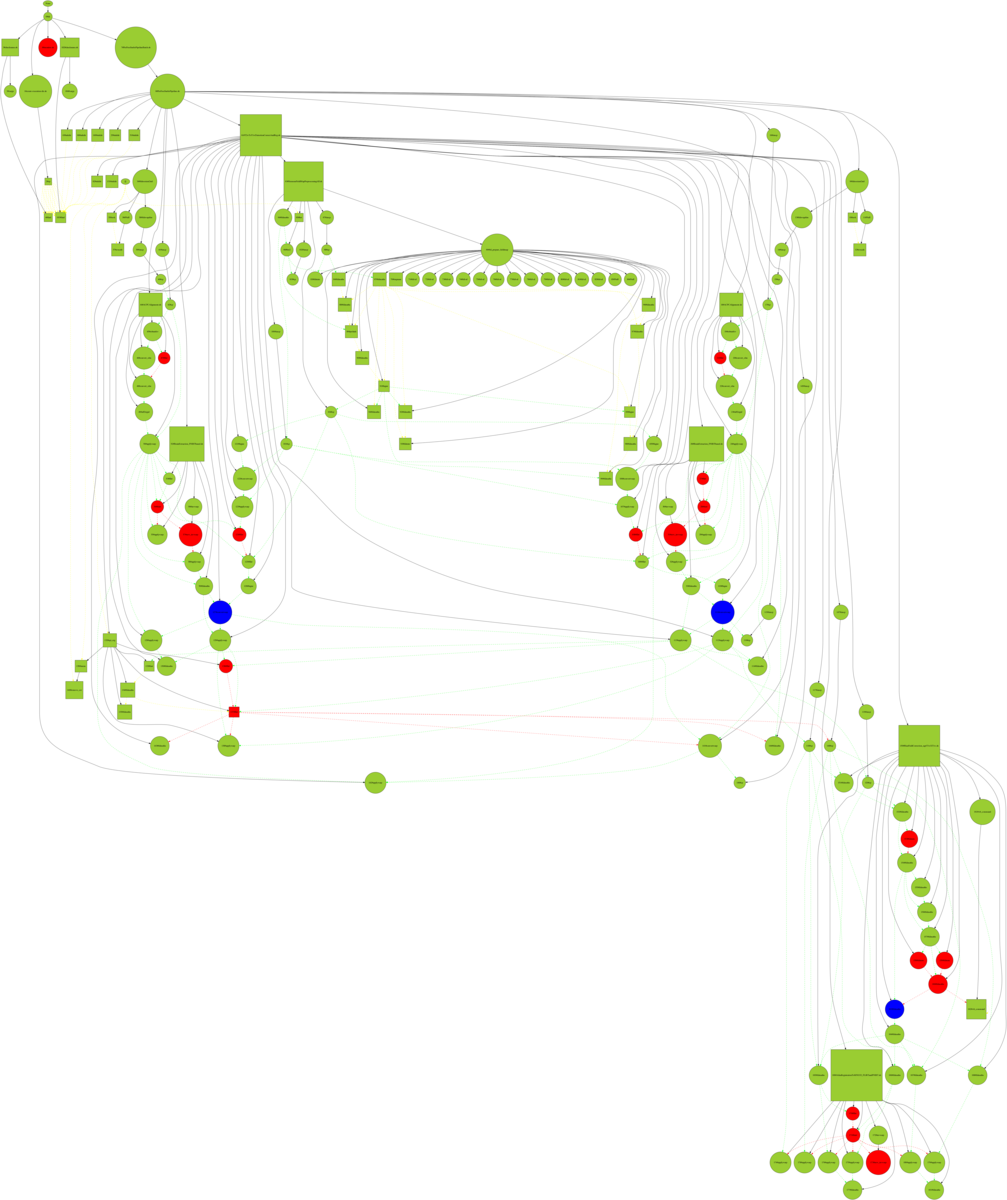
\includegraphics[width=.9\textwidth]{images/graph}
  \caption{A complete process graph from the PreFreesurfer pipeline.
Full-resolution image available at \url{https://drive.google.com/open?id=174yyn8SuVOUcK5aRVw0bagjDanLD0FLt}.}
  \label{fig:complete-graph}
\end{figure*}

\begin{figure*}
\centering
  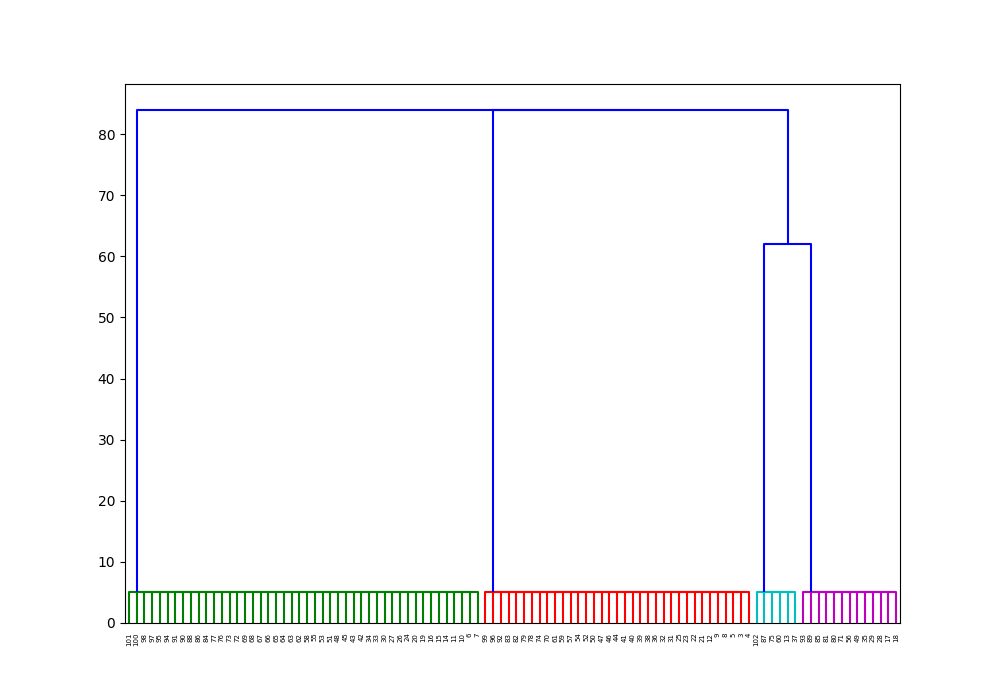
\includegraphics[width=.8\textwidth]{images/hclusters}
  \caption{Different data types clustered among 100 subjects.}
  \label{fig:subj-clusters}
\end{figure*}



\bibliographystyle{plain}
\bibliography{biblio}


\end{document}
